% !TEX root = knottedMain.tex
\documentclass[varwidth=\maxdimen]{standalone}

\usepackage{mathtools,amssymb,mathrsfs,dutchcal,upgreek,faktor,accents,etoolbox,multicol}
\usepackage[dvipsnames]{xcolor}
\definecolor{mygreen}{RGB}{	8,156,79 }
\usepackage{tikz,tikz-cd}
\usetikzlibrary{patterns,knots,arrows.meta,decorations.markings}
\tikzset{>={Straight Barb[scale=0.85]}}
\tikzcdset{
  cells={font=\everymath\expandafter{\the\everymath\displaystyle}},
  arrow style=tikz,
  diagrams={>={Straight Barb[scale=0.85]}},
  every label/.append style = {font = \small}
}


\begin{document}

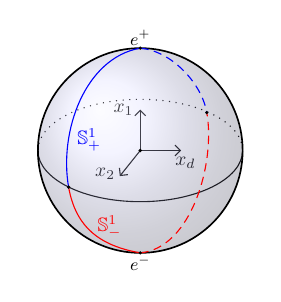
\begin{tikzpicture}[scale=1.3,every node/.style={scale=0.7}]
\clip (-1.1,-1.2) rectangle (1.1,1.2);
    \draw[->] 
        (0,0) -- (0,0.4) node[left]{$x_1$};
    \draw[->] 
        (0,0) -- (0.4,0) node[below, pos=1.1]{$x_d$};
`   \draw[->] 
        (0,0) -- (-0.2,-0.25) node[left, pos=0.9]{$x_2$};
        
    \draw[black] (-1,0) arc (180:360:1cm and 0.5cm);
    \draw[black,dotted] (-1,0) arc (180:0:1cm and 0.5cm);
    \shade[ball color=blue!20!,opacity=0.3] (0,0) circle (1cm);
    \draw[black,semithick] (0,0) circle (1cm);
    \fill (0,0) circle (0.5pt) ;


    \draw[blue]
        (0,1) to[out=-170,in=100,distance=0.55cm] (-0.7,-0.358) ;
    \draw[blue,densely dashed]
        (0,1) to[out=-5,in=100,distance=0.3cm] 
        (0.65,0.37);

    \draw[red]
        (0,-1) to[out=170,in=-80,distance=0.4cm] (-0.7,-0.358) ;
    \draw[red,densely dashed]
        (0,-1) to[out=5,in=-80,distance=0.5cm] 
        (0.65,0.37);
        
    \fill
        (0,1)   circle (0.5pt) 
                node[above=-2pt]{\small$e^+$}
        (0,-1)  circle (0.5pt) 
                node[below=-2pt]{\small$e^-$}
        (-0.7,-0.358) circle (0.5pt)
        (0.65,0.37) circle (0.5pt)
        (-0.5,0.1) node[blue]{$\mathbb{S}^1_+$}
        (-0.3,-0.75) node[red]{$\mathbb{S}^1_-$};

\end{tikzpicture}


\end{document}